\chapter{Expérimentations et Discussion}
\section{Compression}


Les résultats obtenus lors de la compression illustrent l'efficacité de la méthode proposée pour identifier les points caractéristiques d'une trajectoire. En effet, cette méthode nous permet d'atteindre une réduction moyenne de 67.9\% de toutes nos trajectoires. Ces résultats soulignent l'importance de notre approche pour la compression de trajectoires, tout en maintenant leur qualité, comme illustré ici~\ref{fig:traj_versus}.

\begin{figure}[h!]
    \centering
    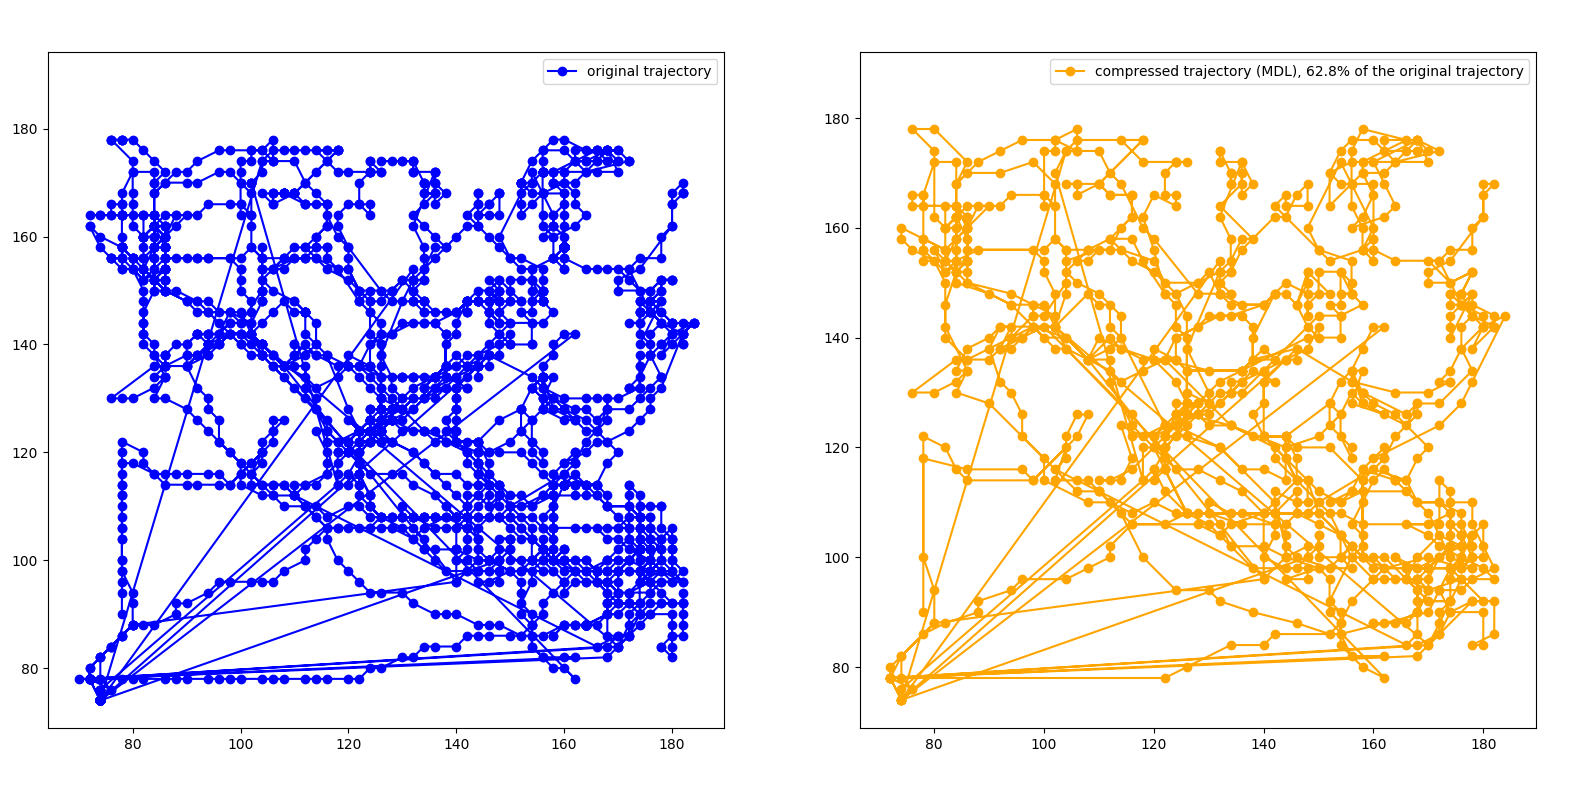
\includegraphics[width=0.8\textwidth]{Images/compVSorigAll.png}
    \caption{Exemple d'une trajectoire avant et après compression}
    \label{fig:traj_versus}
\end{figure}

Il est possible d'observer plus finement l'équilibre entre concision et précision que permet cette méthode sur la figure suivante~\ref{fig:traj_versus100}.

\begin{figure}[h!]
    \centering
    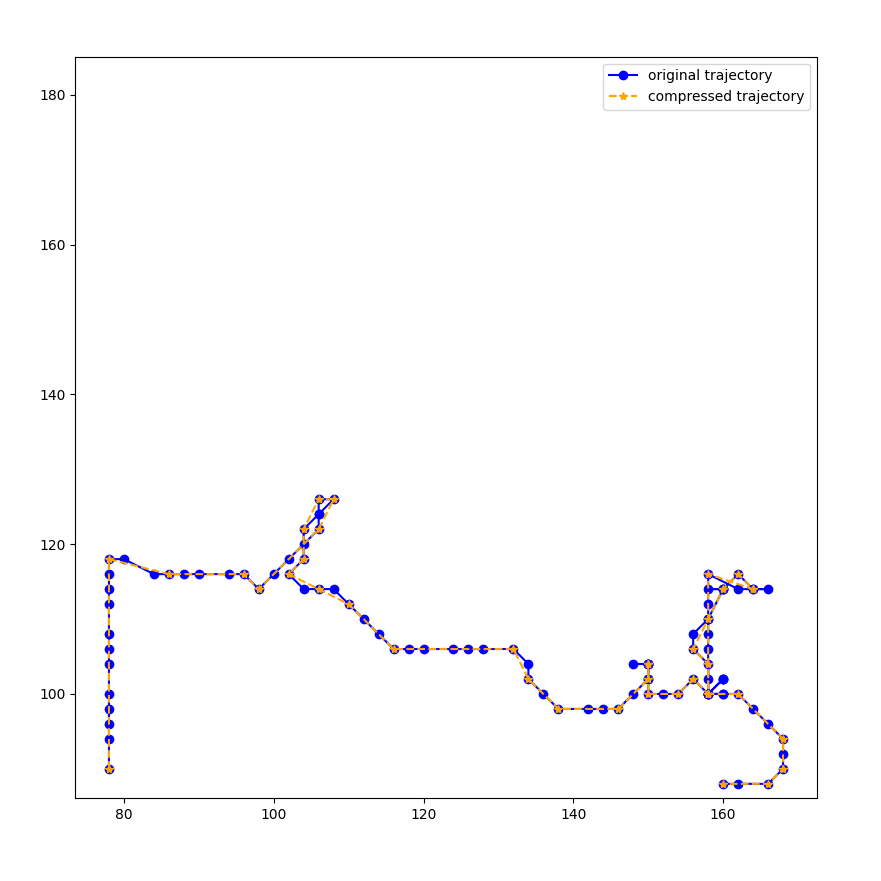
\includegraphics[width=0.5\textwidth]{Images/compVSoriginal100.png}
    \caption{Exemple de la compression sur les 100 premiers points d'une trajectoire}
    \label{fig:traj_versus100}
\end{figure}
\newpage
\section{Clustering}

%Le clustering est une technique d'apprentissage automatique qui consiste à regrouper des données similaires en fonction de leur proximité les unes des autres. 
Pour réaliser un clustering de qualité, il faut d'abord se pencher sur l'étude des paramètres existants. Dans notre cas, il s'agira de l'évaluation de la distance entre deux segments orientés et du nombre de clusters.

Afin d'illustrer plus parlant, il a été décider de se concentrer uniquement sur les trajectoires de l'équipe de gauche.

\textbf{Note}~: Les résultats obtenus avec la méthode de propagation d'affinité présentent un biais significatif en raison de sa complexité spatiale et temporelle, qui suit une complexité en $O(n^2)$. Ainsi, même après compression, le volume important de segments rend difficile son exécution pour plus de deux parties.

\subsection{Paramétrisation de la distance entre segments}

La distance utilisée est la somme pondérée de trois distances~: distance angulaire, distance perpendiculaire et distance parallèle. Les coefficients de cette somme ayant un impact significatif sur les résultats de cette partie, il est nécessaire d'évaluer, de trouver le paramétrage le plus pertinent. 

Pour cette partie, il a été choisi de fixer le nombre de clusters à 100 pour k-means et k-medoids. Il a été remarqué que cela n'avait pas d'impact particulier sur le paramétrage de la distance.

Pour y arriver, plusieurs expérimentations ont été menées successivement afin d'observer les variations qu'impliquent les paramètres pour chaque algorithme. Une fois ce tour d'horizon réalisé, il est possible d'orienter les choix plus précisément. 

\subsubsection{k-means}



\begin{figure}[h!]
    \centering
    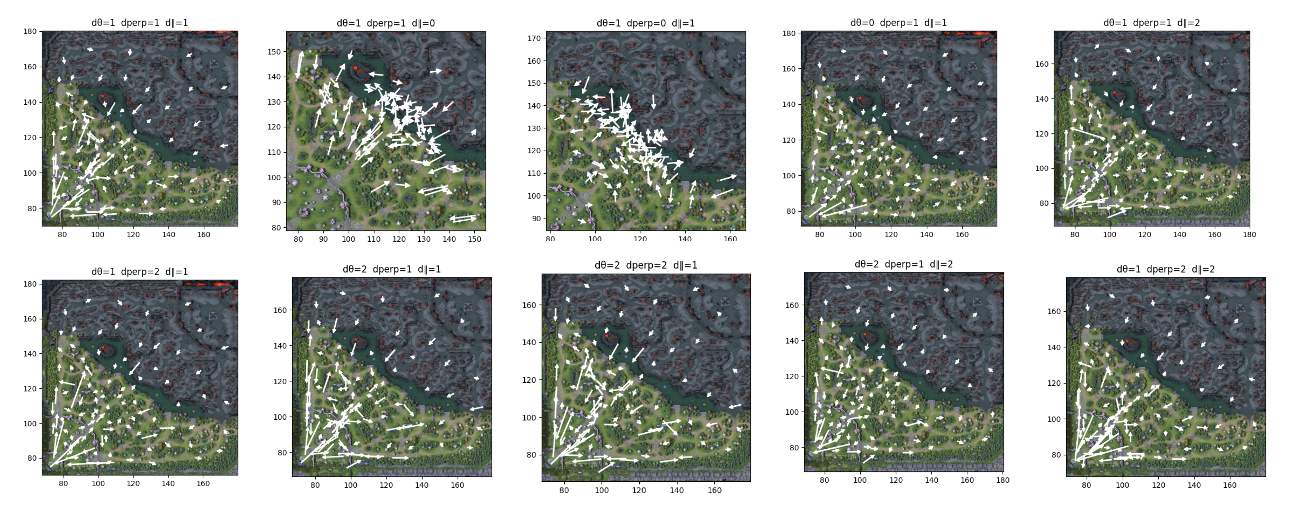
\includegraphics[width=0.9\textwidth]{Images/kmeans/kmeans_seq.png}
    \caption{Résultats clustering k-means pour différentes paramétrisations de la distance}
    \label{fig:kmeans_seq}
\end{figure}

Sur ces résultats \ref{fig:kmeans_seq}, il est possible de distinguer nettement les différences existantes entre chacune des paramétrisations. Lorsque son facteur est égal à 0, a distance angulaire est critique pour obtenir des résultats couvrant correctement les trajectoires sur toute la carte. C'est également le cas pour la distance perpendiculaire. Concernant la distance parallèle, il semblerait qu'elle permette d'affiner le groupement de segments de même orientation et obtenir des segments représentatifs plus longs sur les morceaux de trajectoire récurrents. Cet équilibrage est ici le plus pertinent avec l'adoption d'un facteur 1/2 pour la distance parallèle.

En partant de ces observations, il est apparu qu'un facteur de 1/5 pour la distance parallèle et de 1 pour les deux autres distances donnait des résultats satisfaisant  Comme illustré ici \ref{fig:kmeans_5_5_1}.

\begin{figure}[h!]
    \centering
    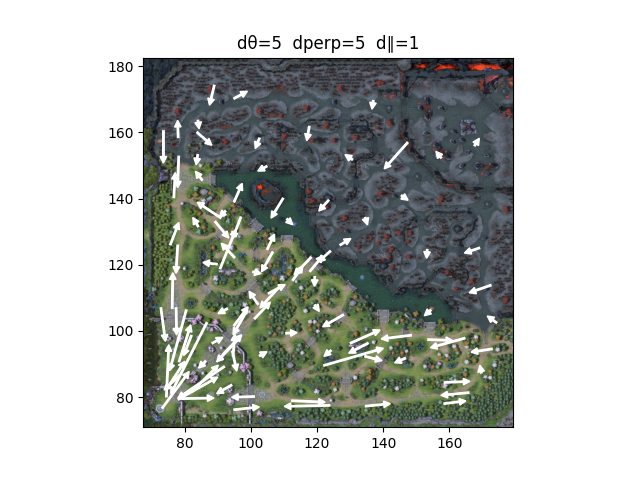
\includegraphics[width=0.6\textwidth]{Images/kmeans/kmeansdBis_5_5_1.png}
    \caption{Résultat clustering k-means avec un facteur parallèle de 1/5}
    \label{fig:kmeans_5_5_1}
\end{figure}


\newpage
\subsubsection{k-medoid}
\begin{figure}[h!]
    \centering
    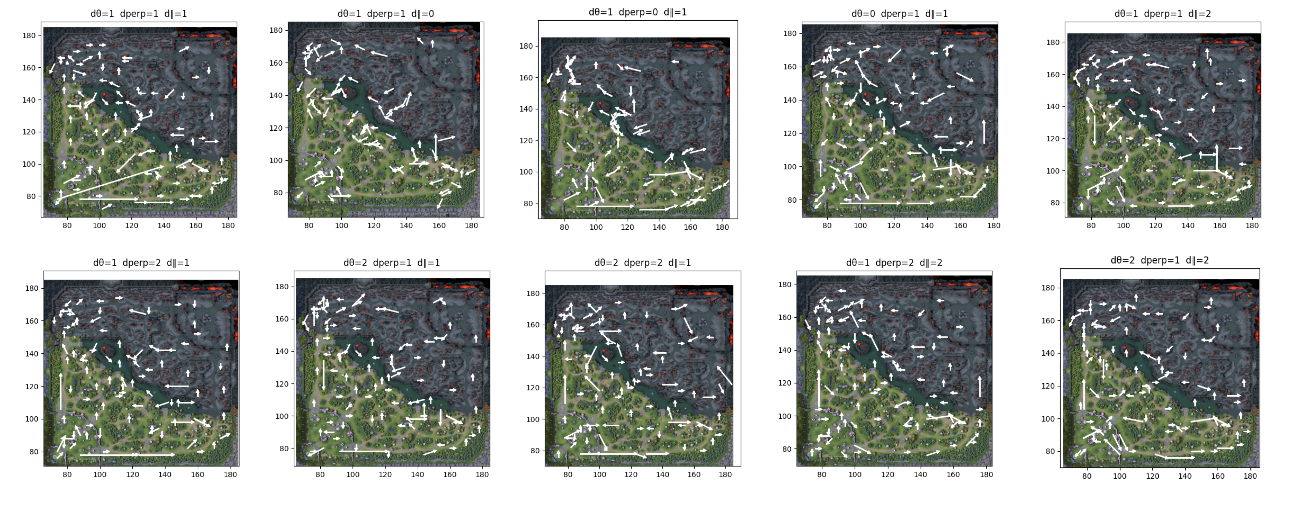
\includegraphics[width=0.9\textwidth]{Images/kmedoid/kmedoid_variationsV2.png}
    \caption{Résultats clustering k-medoids pour différentes paramétrisations de la distance}
    \label{fig:kmed_seq}
\end{figure}

Les résultats des tests \ref{fig:kmed_seq} ont montré que le clustering effectué par k-medoid reste relativement constant. Les trois distances jouent un rôle crucial et aucune des trois ne vraiment être négligée. \\
La distance parallèle et perpendiculaire jouent le rôle le plus important en permettant une distribution plus homogène des clusters sur la carte. En effet, elles permettent la prise en compte de trajectoires représentants des mouvements directes sur une durée plus grande\\
La distance angulaire  permet une meilleure différentiation des trajectoires de direction proches.

Au vu de ces résultats, il semble que partir sur un quasi-équilibre entre les trois distances est la meilleure stratégie à adopter afin d'obtenir les meilleurs résultats \ref{fig:kmed_op}.
\begin{figure}[h!]
    \centering
    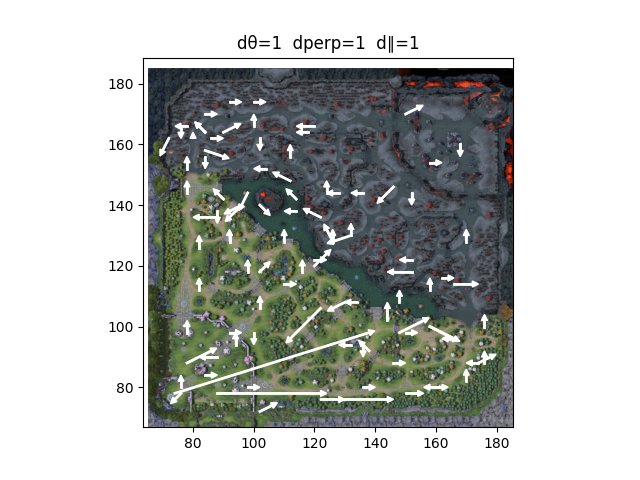
\includegraphics[width=0.6\textwidth]{Images/kmedoid/kmed1_1_1_1.png}
    \caption{K-medoids avec un parametrage de 1 1 1}
    \label{fig:kmed_op}
\end{figure}


\subsubsection{propagation d'affinité}

Pour propagation d'affinité, les résultats \ref{fig:propa_seq} sont globalement assez similaires et traduisent davantage une notion de position que de partitions de trajectoire. En effet, les segments sont généralement courts et répartis sur l'ensemble de la carte de façon homogène. De plus, il y a une tendance à obtenir des segments caractéristique qui sont verticaux, horizontaux ou diagonal.

Néanmoins, il faut prendre en compte que ces résultats sont sujets au biais du faible nombre de parties. De la même façon, cet algorithme possède des paramètres propres, comme le damping, mesure d'acceptance, qui vient affecter le nombre de clusters trouvé.

Ici, il a été choisir d'utiliser un damping de 0.9 avec 60 itérations pour chaque expérimentation.

\begin{figure}[h!]
    \centering
    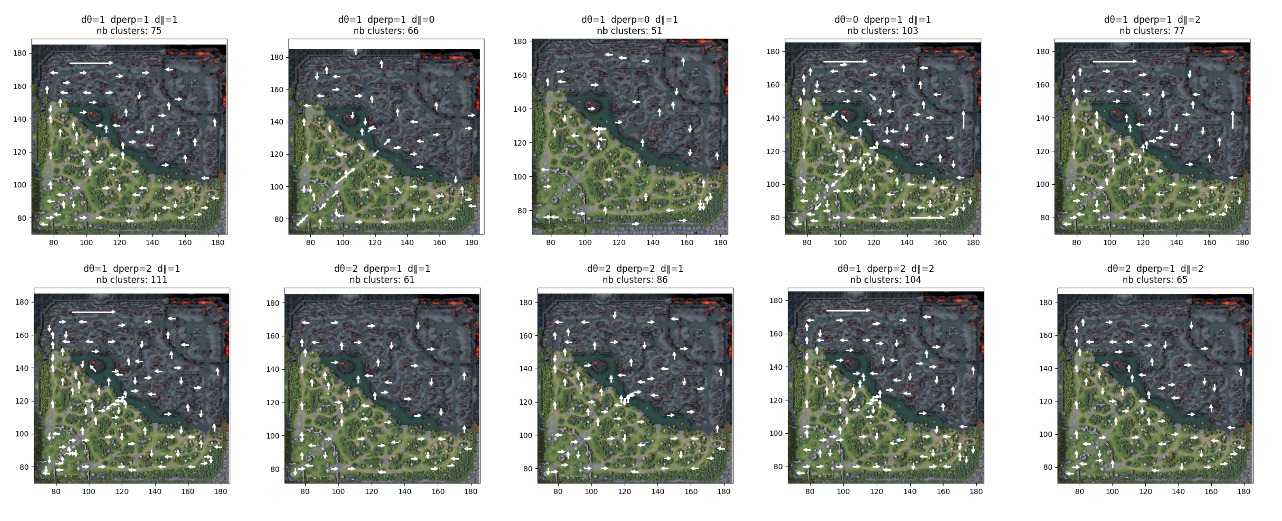
\includegraphics[width=0.9\textwidth]{Images/propa/propa_variations.png}
    \caption{Résultats clustering propagation d'affinités pour différentes paramétrisations de la distance}
    \label{fig:propa_seq}
\end{figure}

Au vu de ces résultats, le plus pertinent reste la mise à 0 du facteur d'angle, comme sur la figure \ref{fig:propa_011}.

\begin{figure}[h!]
    \centering
    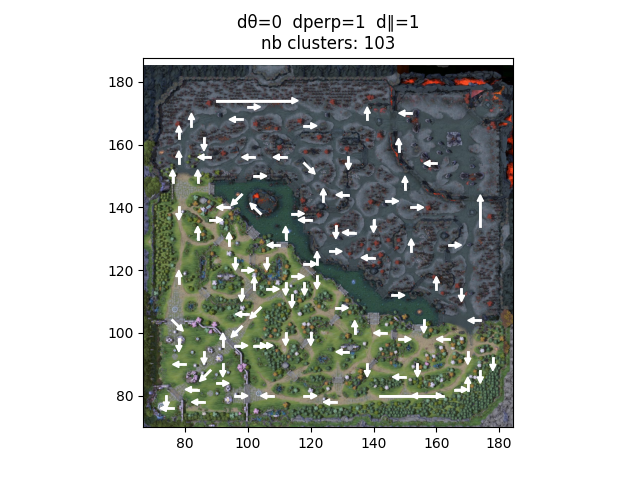
\includegraphics[width=0.6\textwidth]{Images/propa/propa4_0_1_1.png}
    \caption{Résultat clustering propagation d'affinité avec un facteur d'angle de 0}
    \label{fig:propa_011}
\end{figure}



\subsubsection{Discussion}

Il est notable que la paramétrisation a des effets différents sur chacune des méthodes. Cela est assez étonnant dans le cas de k-means et k-medoids, mais la différence s'explique par la différence fondamentale entre les deux algorithmes, ce qui donne aussi sa qualité à k-medoids.

Il est cependant difficile de les comparer avec propagation d'affinités, car celui-ci va également faire une estimation du nombre correct de clusters, en plus de son biais initial lié à son nombre de parties traitées.
% A VERIFIER AVEC LES RESULTATS DEMAIN MATIN

Également, il est intéressant d'observer les différences dans les représentations des trajectoires de chaque côté de la carte, avec des petits segments dans la moitié de carte ennemi (droite), et de longs segments orientés à gauche. Les courts segments semblent représenter des positions sur un espace de la carte \ref{fig:short}. Tandis que les segments orientés allongés semble représenter des trajectoires fréquentes avec une direction précise \ref{fig:long}. 

\begin{figure}[h!]
     \centering
     \begin{subfigure}[b]{0.4\textwidth}
         \centering
         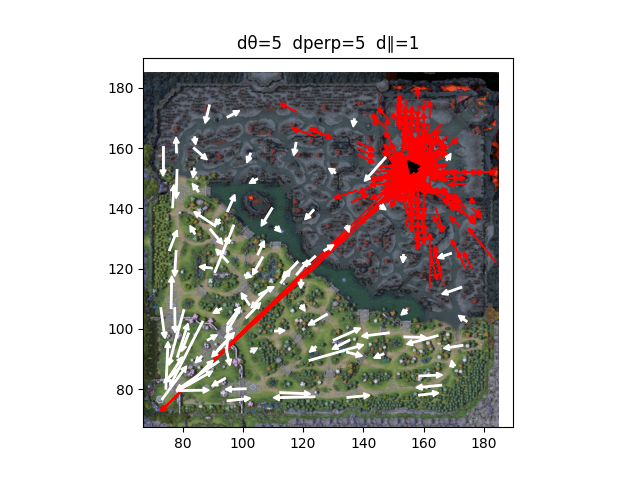
\includegraphics[width=\textwidth]{Images/kmeans/kmeansdBis_show_cluster_short.png}
         \caption{k-means}
         \label{fig:kmean_short}
     \end{subfigure}
     \hfill
     \begin{subfigure}[b]{0.4\textwidth}
         \centering
         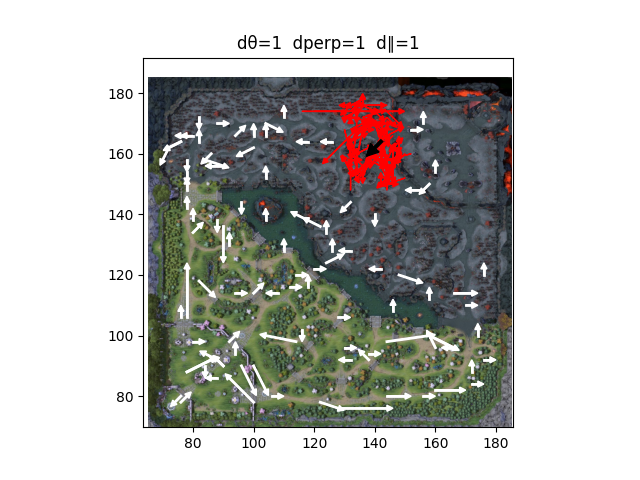
\includegraphics[width=\textwidth]{Images/kmedoid/kmed_212_show_cluster_short.png}
         \caption{k-medoids}
         \label{fig:kmed_short}
     \end{subfigure}
     
     En noir le représentant et en rouge les représentés.
     \caption{Illustration d'un représentant jugé "positionnel"}
     \label{fig:short}
\end{figure}

\begin{figure}[h!]
     \centering
     \begin{subfigure}[b]{0.4\textwidth}
         \centering
         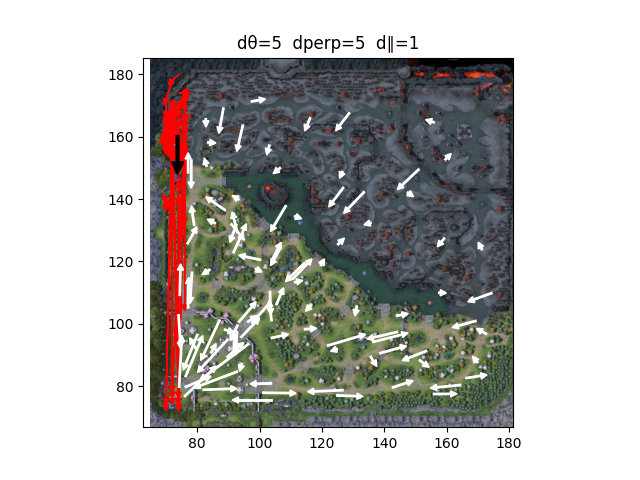
\includegraphics[width=\textwidth]{Images/kmeans/kmeans_long_traj.png}
         \caption{k-means}
         \label{fig:kmean_long}
     \end{subfigure}
     \hfill
     \begin{subfigure}[b]{0.4\textwidth}
         \centering
         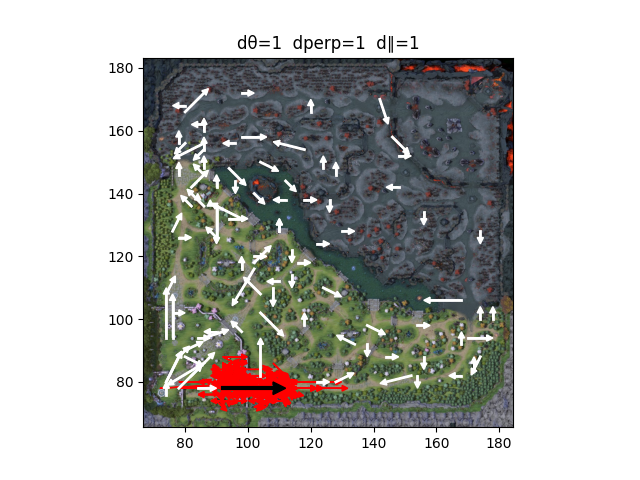
\includegraphics[width=\textwidth]{Images/kmedoid/kmed_long_traj.png}
         \caption{k-medoids}
         \label{fig:kmed_long}
     \end{subfigure}

     En noir le représentant et en rouge les représentés.
     \caption{Illustration d'un représentant de trajectoires}
     \label{fig:long}
\end{figure}
% tmp sans propa

% tmp sans propa

En terme d'information de jeu, il est possible d'interpréter ces différences. Quant aux trajectoires possibles de chaque côté de la carte, cela s'explique pour deux raisons~: premièrement, il est normal pour une équipe de rester de son côté de la carte. Deuxièmement, cela peut s'expliquer par le fait que les excursions du côté adverse de la carte se fait moins souvent et sous la contrainte des déplacements des adversaires, ce qui les rend moins réguliers et moins précis d'une partie à l'autre. 


\subsection{Paramétrisation du nombre de clusters}

Les algorithmes de k-clusters tels que k-means et k-medoids ont un inconvénient notable : ils nécessitent la spécification préalable du nombre de clusters souhaités, ce qui peut entraîner des résultats insatisfaisants en raison de la difficulté à déterminer le nombre optimal de clusters et à choisir une discrétisation adaptée. Bien que l'algorithme de propagation d'affinité soit une alternative intéressante à ce problème, il est difficile de comparer ses résultats avec ceux des autres algorithmes, en raison des différences dans la paramétrisation des distances et du nombre de clusters, comme l'ont montré les résultats précédents.

% L'inconvénient notable des algorithmes de k-clusters, comme k-means et k-medois, est qu'il faut spécifier soit même les nombres de clusters voulus à l'avance. Ce n'est pas optimal, car cela implique souvent de chercher à tâtons, sans garanti de trouver quelque chose de satisfaisant, soit de réaliser une discrétisation trop forte ou trop faible. C'est normalement ici que propagation d'affinité est un algorithme intéressant. Cependant, au vu des résultats précédents sur la paramétrisation des distances qui illustre les différences entre les algorithmes, sans même parler du nombre de clusters, il va être difficile de comparer ces résultats. 

%Une fois avoir déterminé la direction à prendre sur choix des paramètres de la distance, l'étape suivante consiste à déterminer le nombre de clusters permettant d'avoir des résultats de plus grande pertinence.

%\textbf{Note}~: cette partie ne traite pas de la propagation d'affinité, car cet algorithme calcule automatiquement le nombre de clusters à utiliser. Toutefois, il est intéressant de noter que lors de nos expérimentations, nous avons observé une tendance à la diminution puis à la stabilisation du nombre de clusters avec l'augmentation du nombre d'itérations.

Il a été choisi de prendre les meilleurs paramètres de distance pour chaque algorithme pour obtenir une évaluation plus intéressante pour chacun de ces cas.

\subsubsection{k-means}

Au vu des résultats de la figure \ref{fig:kmean_nb}, il est visible qu'à partir de 200 clusters, plusieurs représentants se chevauchent, rendant la discrétion moins intéressante. Cependant, un bon équilibre semble atteint pour un nombre de 150 clusters (figure \ref{fig:kmeans_150}), où il est possible de suivre les trajectoires fréquentes sans que la carte, sans observer trop de chevauchements sur représentants.

\begin{figure}[h!]
     \centering
     \begin{subfigure}[b]{0.35\textwidth}
         \centering
         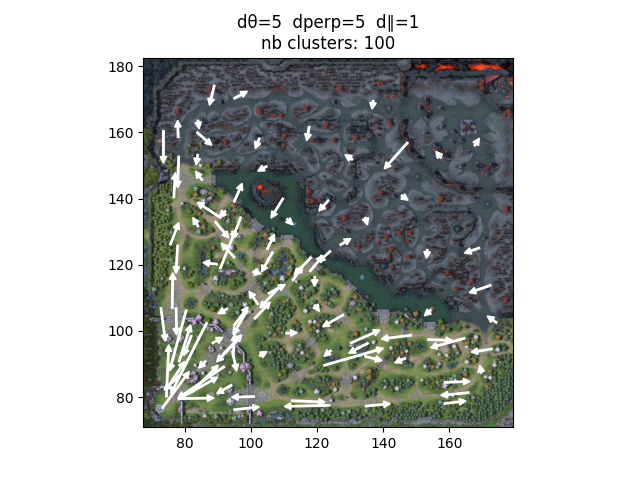
\includegraphics[width=\textwidth]{Images/kmeans/kmeans_100.png}
         \caption{100 clusters}
         \label{fig:kmean_100}
     \end{subfigure}
     %\hfill
     \begin{subfigure}[b]{0.35\textwidth}
         \centering
         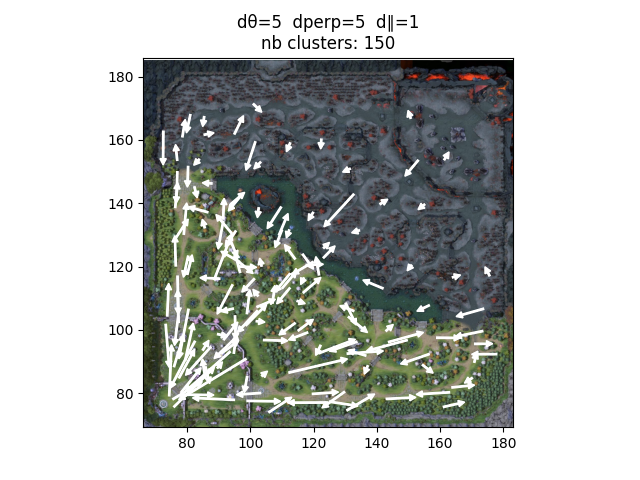
\includegraphics[width=\textwidth]{Images/kmeans/kmeans_150.png}
         \caption{150 clusters}
         \label{fig:kmeans_150}
     \end{subfigure}
     \begin{subfigure}[b]{0.35\textwidth}
         \centering
         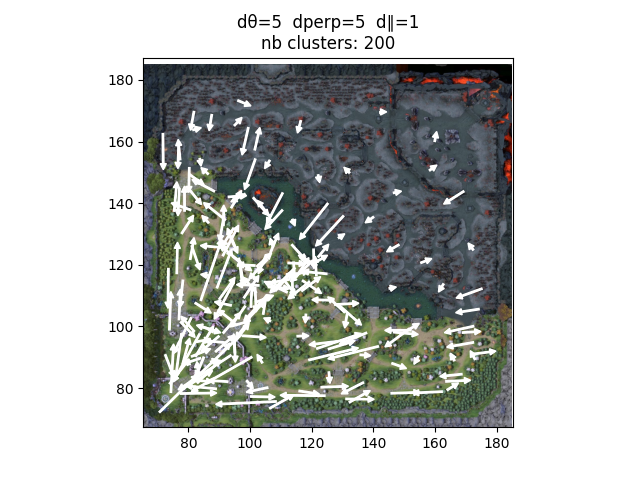
\includegraphics[width=\textwidth]{Images/kmeans/kmeans_200.png}
         \caption{200 clusters}
         \label{fig:kmean_200}
     \end{subfigure}
     %\hfill
     \begin{subfigure}[b]{0.35\textwidth}
         \centering
         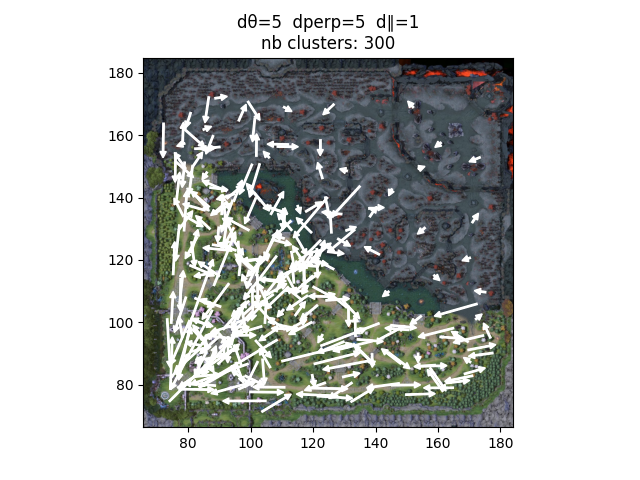
\includegraphics[width=\textwidth]{Images/kmeans/kmeans_300.png}
         \caption{300 clusters}
         \label{fig:kmeans_300}
     \end{subfigure}
     \caption{Évolution de k-means en fonction du nombre de clusters}
     \label{fig:kmean_nb}
\end{figure}


\subsubsection{k-medoids}

Les résultats \ref{fig:kmed_nb} montrent que la qualité de l'information tirée des clusters s'améliore avec leur nombre, mais au-delà de 200 clusters, la quantité d'informations devient trop importante pour en tirer des conclusions. Ainsi, un nombre de 200 clusters semble être un compromis acceptable pour k-medoids afin de suivre l'évolution des trajectoires et détecter les zones à forte fréquentation.
\begin{figure}[h!]
     \centering
     \begin{subfigure}[b]{0.24\textwidth}
         \centering
         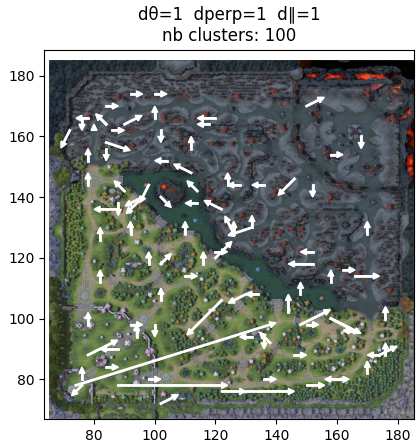
\includegraphics[width=\textwidth]{Images/kmedoid/kmed_100.png}
         \caption{100 clusters}
         \label{fig:kmed_100}
     \end{subfigure}
     \hfill
     \begin{subfigure}[b]{0.24\textwidth}
         \centering
         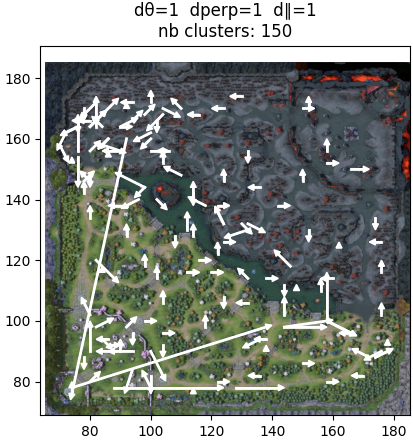
\includegraphics[width=\textwidth]{Images/kmedoid/kmed_150.png}
         \caption{150 clusters}
         \label{fig:kmed_150}
     \end{subfigure}
     \hfill
     \begin{subfigure}[b]{0.24\textwidth}
         \centering
         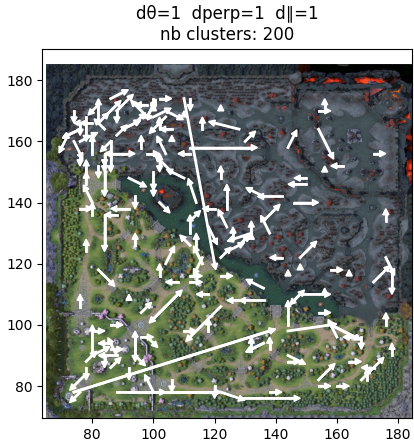
\includegraphics[width=\textwidth]{Images/kmedoid/kmed_200.png}
         \caption{200 clusters}
         \label{fig:kmed_200}
     \end{subfigure}
     \hfill
     \begin{subfigure}[b]{0.24\textwidth}
         \centering
         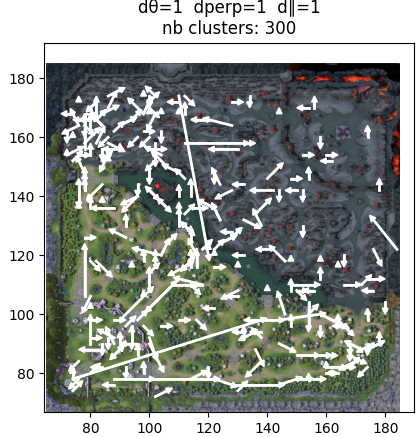
\includegraphics[width=\textwidth]{Images/kmedoid/kmed_300.png}
         \caption{300 clusters}
         \label{fig:kmed_300}
     \end{subfigure}
     \caption{Évolution de k-medoids en fonction du nombre de clusters}
     \label{fig:kmed_nb}
\end{figure}

\subsubsection{propagation d'affinité}

La particularité de propagation d'affinité est justement d'évaluer le nombre de clusters idéal par lui-même. Sur ses meilleurs résultats (figue \ref{fig:propa_011}), nous avons obtenu un nombre de 103 clusters. Cependant, il faut rappeler que ce résultat est aussi lié au facteur de damping et au nombre d'itérations, que nous n'avons pas fait varier. 

\subsubsection{Discussion}

Là encore, les résultats optimaux pour chacun des algorithmes diffèrent. Cela s'explique par leurs différences de paramétrage qui vont influer sur leur définition de représentants. 

Malgré tout, concernant k-means et k-medoids, cela illustre d'autant plus leur différence de fonctionnement, en effet, la capacité de k-medoid à converger qualitativement sur des trajectoires fréquentes font qu'il est possible d'affiner la discrétisation sans brouiller nos résultats. 

L'idéal aurait été d'utiliser la capacité de propagation à trouver le nombre correct de clusters, mais cela s'avère difficile ici. En effet, il aurait fallu que les algorithmes possèdent un paramétrage optimal équivalent. De plus, il aurait fallu à la fois surmonter la contrainte matérielle pour utiliser pleinement propagation d'affinité et mener une étude sur le facteur optimal de damping à utiliser.

\section{Extraction séquentielle}
\subsubsection{Paramètres de l'extraction}
L'algorithme d'extraction séquentiel utilisé \cite{hirate2006generalized} permet l'extraction de motifs fréquents. Plusieurs paramètres rentrent alors en compte.
\begin{enumerate}
    \item \textbf{minsup(minimum support)}~: le nombre minimum de transactions ou doivent apparaître un motif fréquent.
    \item \textbf{min\_time\_interval}~: le temps minimal permis séparant deux itemsets successifs dans un motif.
    \item \textbf{max\_time\_interval}~: le temps maximal permis séparant deux itemsets successifs dans un motif.
    \item \textbf{min\_whole\_interval}~: le temps minimal permis séparant le premier itemset et le dernier itemset d'un motif fréquent (taille minimale du motif).
    \item \textbf{max\_whole\_interval}~: le temps maximal permis séparant le premier itemset et le dernier itemset d'un motif fréquent (taille maximale du motif).
\end{enumerate}

\subsection{Résultats}

Concernant l'extraction, beaucoup de paramétrage ont été testés, mais malgré tout, peu de résultats concluants ont pu être obtenus dans le temps imparti. 

Pour commencer, un découpage arbitraire a été expérimenté. De 30 à 120 secondes, pour finalement rester sur une moyenne de 60 secondes. 

Dès lors, nous avons eu des problèmes d'extraction n'ayant pas spécialement d'intérêt où nous avions des morceaux de trajectoires qui ne se suivaient pas du tout et provenant très probablement de 2 joueurs différents, comme illustré sur la figure \ref{fig:extraction_bad}, il a été décidé de se concentrer sur la trajectoire d'un joueur à la fois.

Ensuite, après les obtentions de résultats illustrant très largement des suites successives de la même trajectoire, nous avons voulu faire varier l'intervalle de temps entre chaque transaction étudié dans l'idée d'éviter le cas où la vitesse ou le rythme des positions des joueurs sur chaque morceau de trajectoire rendrait impossible l'extraction de motifs d'une taille supérieure à 2. Comme illustré sur la figure \ref{fig:interval}. Même si cela pourrait engendrer une perte d'information, il a quand même était jugé nécessaire.

\begin{figure}[h!]
     \centering
     \begin{subfigure}[b]{0.44\textwidth}
         \centering
         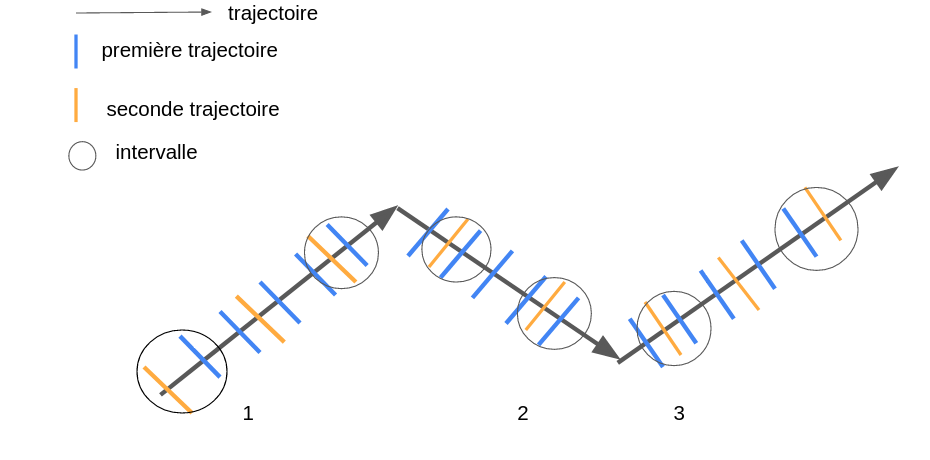
\includegraphics[width=\textwidth]{Images/interval_1.png}         
     \end{subfigure}
     \hfill
     \begin{subfigure}[b]{0.44\textwidth}
         \centering
         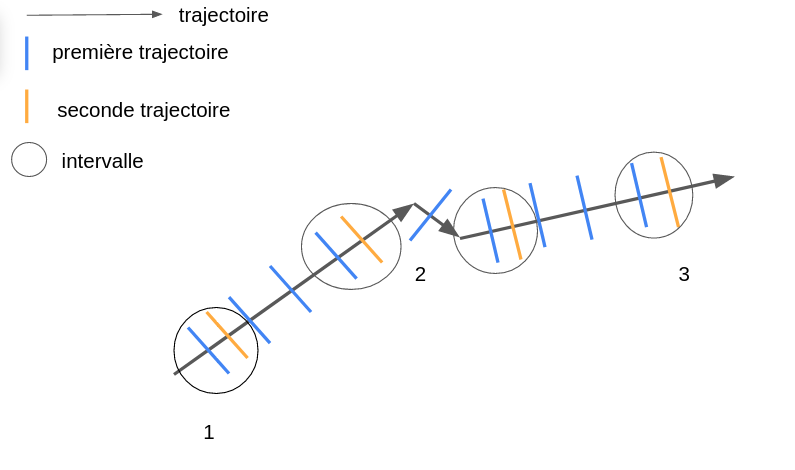
\includegraphics[width=\textwidth]{Images/interval_2.png}
     \end{subfigure}
     \caption{intervalle de temps}
     \label{fig:interval}
\end{figure}     

À ce moment-là, il a été possible d'extraire des motifs formés d'une suite de morceau de trajectoire, exemple figure \ref{fig:extraction_good}, mais ces résultats n'ont pu être obtenus qu'avec un support minimum assez faible (5\%), ce qui n'était pas très satisfaisant. Cependant, il n'était toujours pas possible d'extraire des motifs composés de plus de 2 segments.

\begin{figure}[h!]
     \centering
     \begin{subfigure}[b]{0.44\textwidth}
         \centering
         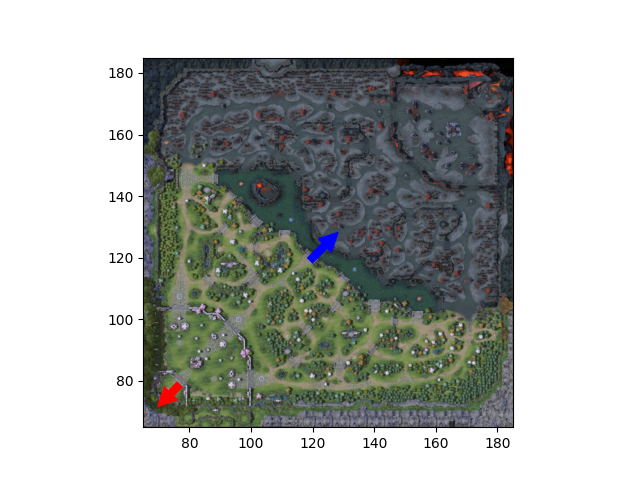
\includegraphics[width=\textwidth]{Images/bad_seq2.png.png}
          \caption{résultat incorrect}
          \label{fig:extraction_bad}
     \end{subfigure}
     \hfill
     \begin{subfigure}[b]{0.44\textwidth}
         \centering
         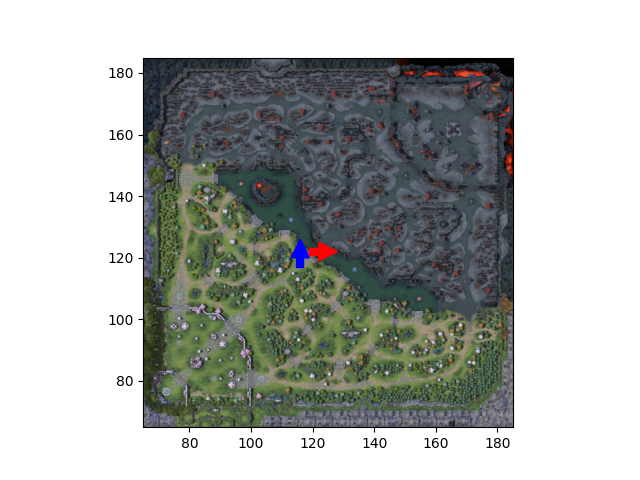
\includegraphics[width=\textwidth]{Images/good_seq2.png.png}
     \caption{Résultat correct}
     \label{fig:extraction_good}
     \end{subfigure}
     \caption{Résultat extraction}
\end{figure}    


\subsection{Discussion} % à voir.

Les résultats obtenus ne sont pas complets et mériteraient d'aller plus loin et d'étudier plus amplement les paramètres disponibles ainsi que le choix du découpage. Par exemple, il serait intéressant d'essayer une extraction sur différents moments des parties (début, milieu de jeu, etc...) afin d'observer directement en fonction de chaque partie les motifs fréquents et de mieux pouvoir les analyser.

De plus, il serait possible d'essayer d'autres méthodes pour extraire des motifs significatifs sans passer par découpage en trajectoire, mais en passant par une discrétisation de la position (exemple : découpage de la carte en une grille de taille n). Et d'ensuite réaliser une extraction sur ces points. L'avantage étant de ne pas passer par l'étape de recodage ni de la compression sous forme de trajectoire et de privilégier l'information positionnelle.